\subsection{If a parent class imports a class from different package, the target child class within same java file cannot be duplicate with that imported class after rename.}

If a parent class imports a class from different package and if we try renaming a child class with the same name as the class imported into its parent class within the same java file, compiler produces the error as ``a compilation unit must not import and declare a type with the same name''~\cite{EclipseWebPage}.This precondition can be explained by the following example.

\begin{figure}[th]
\centering
\begin{minipage}[t]{0.45\linewidth}
\begin{lstlisting}[language=java, basicstyle=\scriptsize\ttfamily,frame=single]	
A.java

package q;
import p.C;

public class A{	
}

class B extends A{	
}

class D extends B{
}
\end{lstlisting}
\centering{(a) Before renaming child class B}
\end{minipage}
\hfill
\begin{minipage}[t]{0.45\linewidth}
\begin{lstlisting}[language=java, basicstyle=\scriptsize\ttfamily,frame=single]
A.java

package q;
import p.C;

public class A{	
}

class C extends A{	
}

class D extends B{
}	
\end{lstlisting}
\centering{(b) After renaming child class  B to C}
\end{minipage}
\caption{\textbf{Precondition for renaming child class within the same java file}}
\label{figure:figpc3_1}
\end{figure}

From the above Fig. \ref{figure:figpc3_1}, we see that if a parent class A imports a class C from package `p' and if we try to rename the child class B to C or D to C, java generates compile error as shown in the Fig. \ref{figure:figpc3_2}. As mentioned in  section \ref{sec:precon2}, the same precondition also holds good for renaming a child class. This precondition is applicable for all ancestor class and we have to trace back and check if any of the parent class is importing a class with same name before renaming the child class within the same java file.
\begin{figure}[htbp]
\centerline{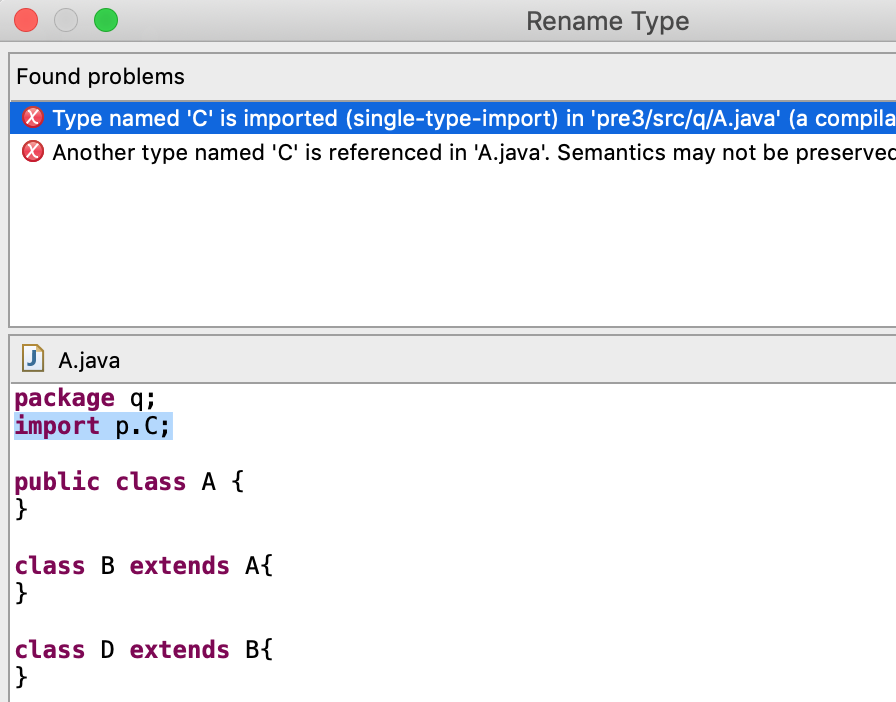
\includegraphics[width=85mm,scale=0.5]{precond3.png}}
\caption{\textbf{Error produced after renaming the child class.}}
\label{figure:figpc3_2}
\end{figure}

If a parent class imports a class from different package and if the child class is defined in a separate java file, then in that case we can refactor and rename the child class to the imported class name.